\chapter{Hardware Design}
\label{ch:hw_design}
\section{Core Design}
We decided to design and implement two unique RocketCore CPUs for the heterogeneous SoC. These will be in two separate tiles with cache coherency. The aim will be for each core to implement the RV64GC ISA, the 'general-purpose' RISC-V ISA, as well as an MMU (Memory Management Unit) in order to run a full Debian Linux OS, if only with terminal interaction. The following code snippets show the parameterisation options available for the RocketCore CPU and the tiles they lie within.

\begin{figure}
    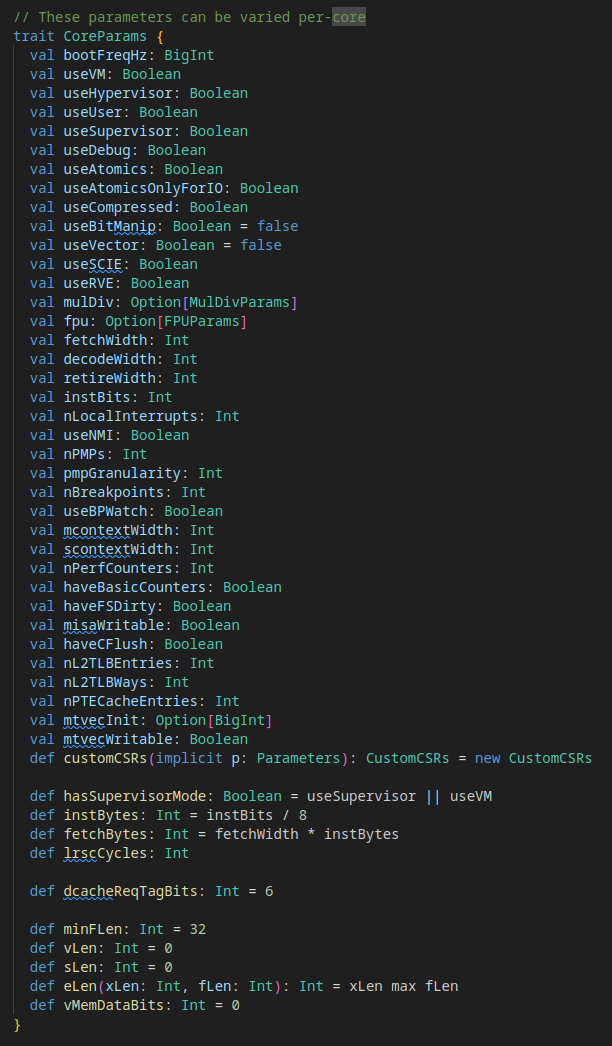
\includegraphics[]{./img/core_params.png}
\end{figure}
\begin{figure}
    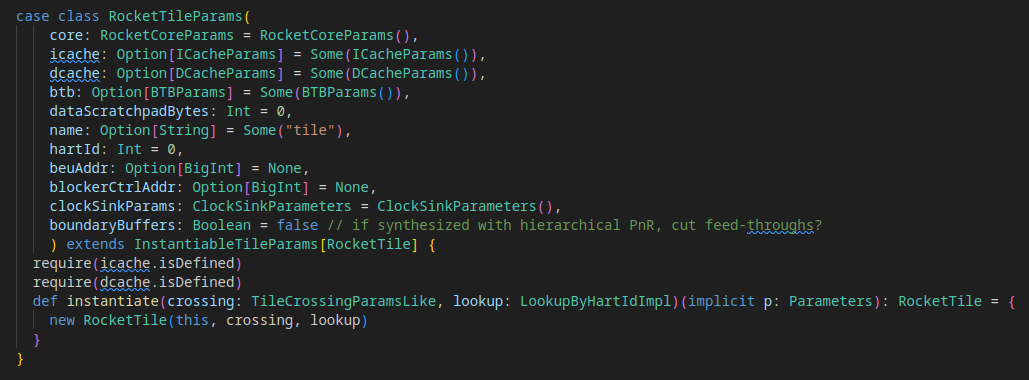
\includegraphics[]{./img/rocket_tile_params.png}
\end{figure}

\subsection{Default RocketCore CPUs}
RocketCore contains some predefined core designs. These allow a user to immediately generate a RocketCore CPU without having to parameterise their own, with a few different options dependant on the use case.

\subsubsection{Small Core}
The RocketCore predefined small core implements the RV64IMAZicsrZifenceiC ISA, removing the single-precision floating point and double-precision floating point instructions from the RV64GC ISA. The point of this is to remove the FPU from the CPU, much reducing the logic required by the design.

\begin{figure}
    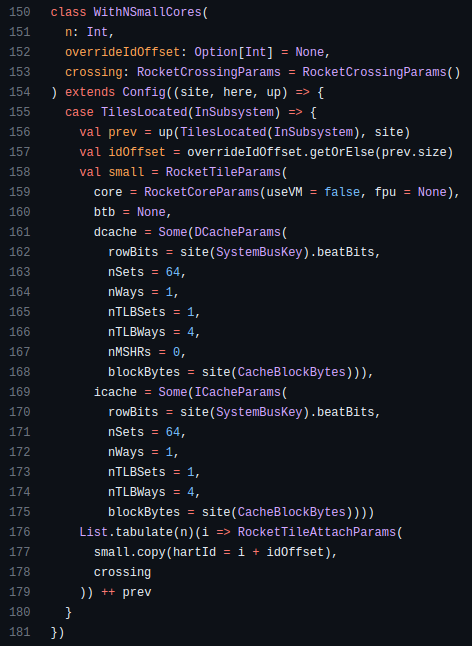
\includegraphics[]{./img/rocketcore_default_small.png}
\end{figure}

The MMU has also been removed from the CPU. This prevents virtual memory from being used, and forces 

\chapter{Test Design}
\label{ch:test_design}

In this chapter, we describe the implementation of the design we described in \Cref{ch:design}. You should \textbf{not} describe every line of code in your implementation. Instead, you should focus on the interesting aspects of the implementation: that is, the most challenging parts that would not be obvious to an average Computer Scientist. Include diagrams, short code snippets, etc. for illustration.